\section{Linear Search}
\subsection{Aim}
To perform linear search on an array of numbers

\subsection{Code}
\begin{lstlisting}
DATA SEGMENT
  arr DW 1000H, 3000H, 4000H, 2000H
  count DW 4
  query DW 3001H
  msg1 DB "Found$"
  msg1len DW $-msg1
  msg2 DB "Not found$"
  msg2len DW $-msg2
DATA ENDS

CODE SEGMENT
ASSUME CS:CODE, DS:DATA
START:
  MOV AX, DATA
  MOV DS, AX
  MOV CX, count
  LEA SI, arr
  XOR AX, AX

SEARCHLOOP:
  MOV AX, query
  CMP AX, [SI]
  JE FOUND
INCRLOOP:
  ADD SI, 2
  LOOP SEARCHLOOP
  JMP NOTFOUND

FOUND:
  LEA DX, msg1
  MOV AH, 09H
  INT 21H
  JMP EXIT

NOTFOUND:
  LEA DX, msg2
  MOV AH, 09H
  INT 21H
  JMP EXIT  

EXIT:
  MOV AH, 4CH
  INT 21H
CODE ENDS
END START
\end{lstlisting}

\subsection{Output}
\begin{center}
	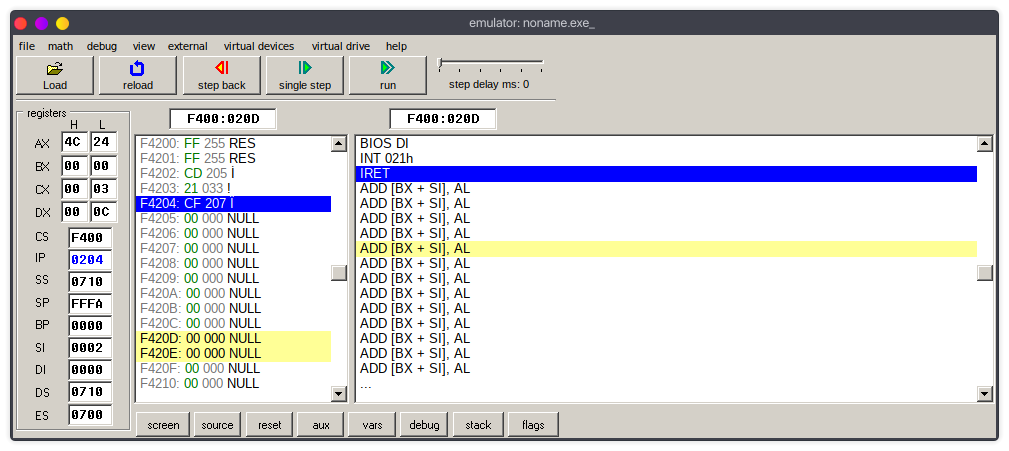
\includegraphics[width=0.90\textwidth]{img/p11/ss1.png}
	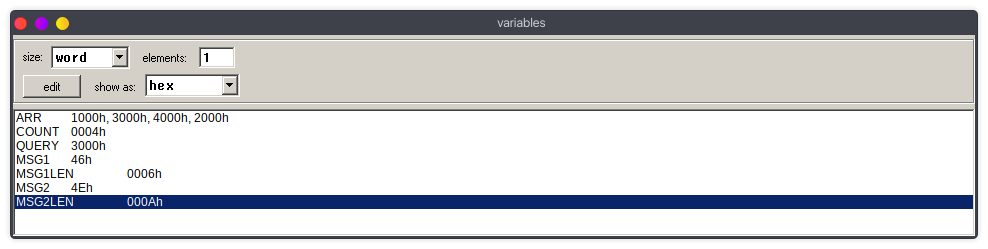
\includegraphics[width=0.90\textwidth]{img/p11/ss2.png}
	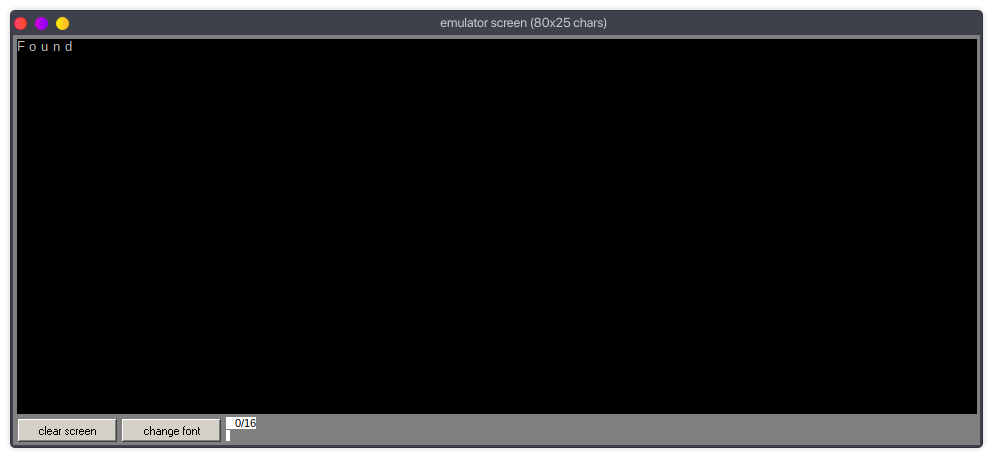
\includegraphics[width=0.90\textwidth]{img/p11/ss3.png}\\
  Output for 3000H\\
  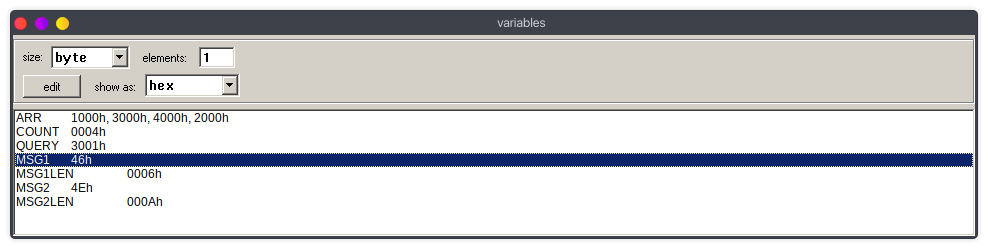
\includegraphics[width=0.90\textwidth]{img/p11/ss4.png}
	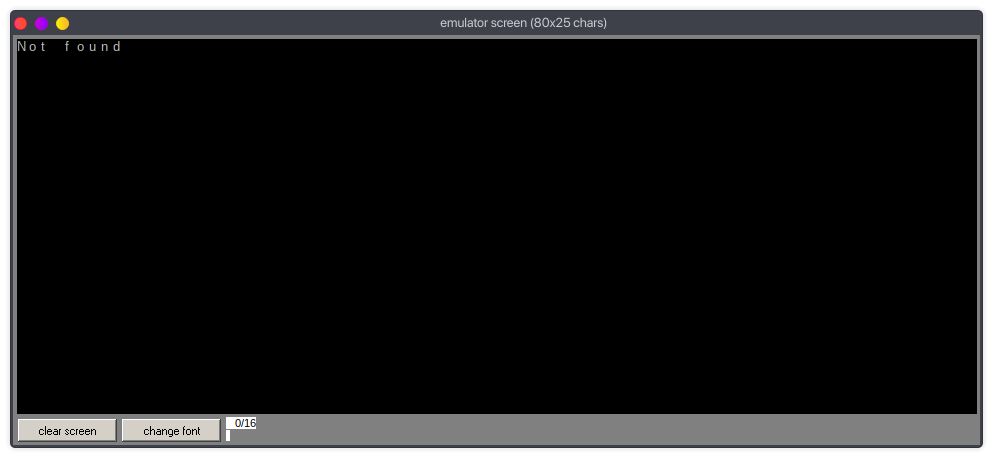
\includegraphics[width=0.90\textwidth]{img/p11/ss5.png}\\
  Output for 3001H
\end{center}

\subsection{Result}
Linear search was performed in an array in emu8086